\documentclass[10pt,twoside]{article}
\usepackage[utf8]{inputenc}
\usepackage{natbib}
\usepackage{graphicx}
\usepackage{booktabs}
\usepackage{adjustbox}
\usepackage[table,xcdraw]{xcolor}
\usepackage{amsmath}
\usepackage[]{todonotes}
\usepackage{fancyhdr}
\usepackage{multirow}
\usepackage{multicol}
% Idioma
\usepackage[english]{babel}

\usepackage[none]{hyphenat}

\usepackage[Alg.]{algorithm}
\usepackage{algpseudocode}

\newcommand{\ignore}[1]{}


\title{Local Search for Heterogeneous Cumulative Capacitated Vehicle Routing Problem}
\author{\emph{David Plazas Escudero}\\
\vspace{0.3cm}
\small{\tt{dplazas@eafit.edu.co}}\\
Departamento de Ciencias Matemáticas\\
Escuela de Ciencias\\
Universidad EAFIT\\
Medellín -- Colombia}
\date{}

\usepackage{anysize}
\marginsize{3cm}{2cm}{2cm}{3cm}

% Configurar encabezado y pie de página
\pagestyle{fancy}
\lfoot[\date{\today}]{\date{\today}}
\rfoot[\thepage]{\thepage}
\cfoot[]{}
\rhead[Plazas (2019)]{Constructive Algorithm for Heterogeneous Cumulative Capacitated Vehicle Routing Problem}
\lhead[]{}

\fancypagestyle{firststyle}
{
   \fancyhf{}
   \fancyfoot[R]{Last updated: September 23, 2019}
}

\sloppy



\begin{document}

\maketitle

\thispagestyle{firststyle}

% \begin{abstract}
% Buenas
% \vspace{0.2cm}\\
% %
% \noindent \textbf{Keywords:}
% Heuristic, constructive algorithm, vehicle routing problem, heterogeneous-fleet.
% \end{abstract}

\section{Algorithm Description}\label{sec_intro}
\subsection{VRP Neighborhood Operators}
The three neighborhood operators considered in this work are based on the description provided in \cite{layeb2013grasp}.
\subsubsection{In-Route 2-Opt}
The first operator considered is the widely used 2-opt for routing problems, this operator takes each possible pair or nodes in a route and checks if swapping two nodes and reversing the route between them is a better alternative in terms of distance traveled. Figure \ref{fig:2opt} illustrates the operator.

\begin{figure}[H]
    \centering
    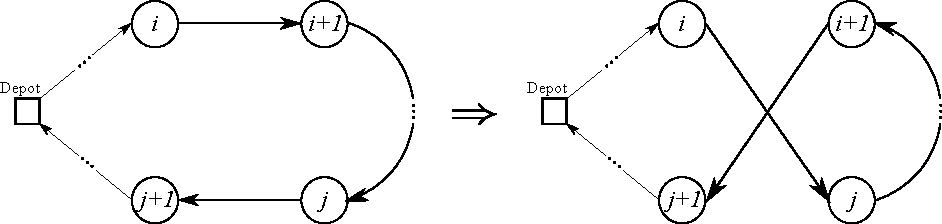
\includegraphics[scale=0.73]{figs/2opt.pdf}
    \caption{2-Opt operator.}
    \label{fig:2opt}
\end{figure}

\subsubsection{Inter-Route 1-1 Exchange}
This operator takes two nodes in two different routes and simply swaps them into the other node's route and checks if the new route makes an improvement in the objective function. This procedure is depicted in Figure \ref{fig:11ex}.

\begin{figure}[H]
    \centering
    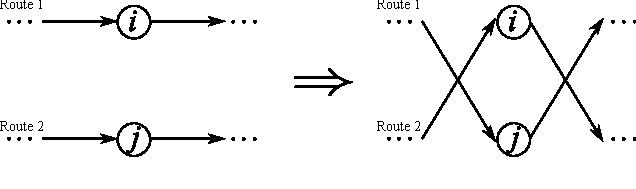
\includegraphics[scale=0.9]{figs/11ex.pdf}
    \caption{1-1 Exchange Operator.}
    \label{fig:11ex}
\end{figure}

\subsubsection{Move Operation}
This method, for each route, takes a node and attempts to insert it in a new position within the same route and, as well, checks if this change makes an improvement in the objective function.

\subsection{Simulated Annealing (SA)}
The algorithm was originally proposed for combinatorial optimization by \cite{kirkpatrick1983optimization}. The pseudo-code for this metaheuristic is shown in Figure \ref{fig:anneal}. The algorithm is widely used due to its ability to diversify the solution by accepting ``bad'' neighbors with a given probability. The most important feature of the SA is that the algorithm starts accepting a ``lot'' of ``bad'' solutions, but as the algorithm runs, the probability of accepting a ``bad'' solution is reduced significantly and one finally accepts better solutions to the current one.

\begin{figure}[H]
    \centering
    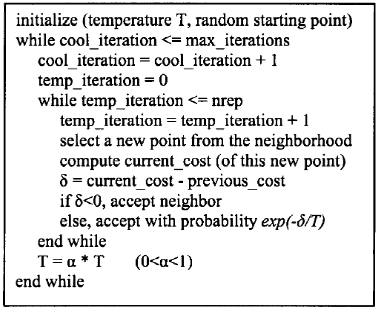
\includegraphics[scale=0.7]{figs/anneal.png}
    \caption{Pseudo-code for SA \citep{ferentinos2002heuristic}.}
    \label{fig:anneal}
\end{figure}

\subsection{Variable Neighborhood Descent (VND)}
Originally proposed in \cite{mladenovic1997variable}, this metaheuristic is widely used nowadays. It was constructed on the following facts \citep{mladenovic1997variable}:
\begin{enumerate}
    \item \textit{``A local minimum with respect to one neighborhood structure is not necessarily so for another'';}
    \item \textit{``A global minimum is a local minimum for all possible neighborhood structures'';}
    \item \textit{``For many problems local minima with respect to one or several neighborhoods are relatively close''.}
\end{enumerate}
Based on this, the VND metaheuristic was developed, which is presented in Figure \ref{fig:vnd}.

\begin{figure}[H]
    \centering
    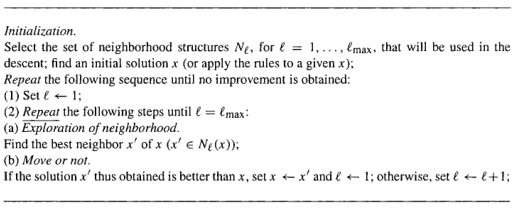
\includegraphics[scale=0.8]{figs/vnd.png}
    \caption{Pseudo-code for VND \citep{mladenovic1997variable}.}
    \label{fig:vnd}
\end{figure}

\section{Results}
The initial solution was constructed with a sweep-based constructive heuristic for VRPs; the original heuristic was proposed in \cite{gillett1974heuristic} and it was adapted for the heterogeneous capacitated case.

For the SA, the implementation was based on the pseudo-code shown in Figure \ref{fig:anneal}, although some different parameters where considered: instead of a \texttt{max\_iterations} parameter, we set a final temperature \texttt{tempf} and the condition on outter-most loop was while the current temperature \texttt{temp} was greater than \texttt{tempf} and the current temperature decreases with a ``cooling'' rate $r$. On the other hand, \texttt{nrep} was not considered; instead, the neighborhood was generated by sampling all possible 2-opt neighbors and including them in the SA neighborhood if a random number was below 0.5 (equivalent to taking half of the complete neighborhood in average). From this neighborhood, we select the one that has the minimum value of the objective function and evaluate the standard procedure for the SA.

For this SA, the final temperature \texttt{tempf} was set to $10^{-3}$, the cooling rate $r=0.65$ and initial temperature to 25. In Table \ref{tab:SA}, the results for the 21 instances are presented. The column \textbf{E.T. (s)} stands for ``execution time'', measured in seconds; and the column \textbf{\%} stands for the percentage of improvement with respect to the initial solution, calculated as follows:
\[
\%:=\dfrac{z_0-z_{{\rm SA}}}{z_0}\times100\%
\]


On the other hand, the VND was implemented based on the pseudo-code shown in Figure \ref{fig:vnd} but it is not executed until to improvement is found. It is executed twice: on each iteration, it finds the local optimum with 2-opt, then applies the 1-1 exchange to this local optimum and finally it applies the move operator to this last optimum. This process is done twice. The results for this procedure are presented in Table \ref{tab:vnd}. This table uses the same convention as for SA.


\begin{table}
\parbox{.45\linewidth}{
\centering
\begin{tabular}{cccc}
\hline
\textbf{Instance} & \textbf{Nodes} & \textbf{\%} & \textbf{E.T. (s)} \\ \hline
1                 & 50             & 36.51       & 1.13              \\
2                 & 50             & 36.03       & 1.35              \\
3                 & 50             & 39.6        & 1.88              \\
4                 & 75             & 21.43       & 1.34              \\
5                 & 75             & 24.83       & 1.54              \\
6                 & 75             & 32.11       & 1.98              \\
7                 & 100            & 37.75       & 7.61              \\
8                 & 100            & 39          & 8.52              \\
9                 & 100            & 45.29       & 9.61              \\
10                & 150            & 49.33       & 17.9              \\
11                & 150            & 41.88       & 19.31             \\
12                & 150            & 43.14       & 19.7              \\
13                & 199            & 49.68       & 21.67             \\
14                & 199            & 47.95       & 21.41             \\
15                & 199            & 41.55       & 14.92             \\
16                & 120            & 56.91       & 30.2              \\
17                & 120            & 58.05       & 10.37             \\
18                & 120            & 57.34       & 10.79             \\
19                & 100            & 16.39       & 4.75              \\
20                & 100            & 17.14       & 5.01              \\
21                & 100            & 20.57       & 5.37              \\ \hline
\end{tabular}
\caption{Results for SA.}
\label{tab:SA}
}
\hfill
\parbox{.45\linewidth}{
\centering
\begin{tabular}{cccc}
\hline
\textbf{Instance} & \textbf{Nodes} & \textbf{\%} & \textbf{E.T. (s)} \\ \hline
1                 & 50             & 50.19       & 0.72              \\
2                 & 50             & 46.08       & 0.6               \\
3                 & 50             & 48.06       & 0.9               \\
4                 & 75             & 43.65       & 1.46              \\
5                 & 75             & 38.81       & 0.77              \\
6                 & 75             & 52.35       & 1.62              \\
7                 & 100            & 49.37       & 4.56              \\
8                 & 100            & 54.36       & 5.19              \\
9                 & 100            & 56.93       & 7.04              \\
10                & 150            & 55.11       & 13.42             \\
11                & 150            & 49.24       & 8.4               \\
12                & 150            & 49.44       & 19.14             \\
13                & 199            & 58.76       & 18.76             \\
14                & 199            & 56.48       & 17.49             \\
15                & 199            & 55.47       & 9.95              \\
16                & 120            & 69.35       & 19.91             \\
17                & 120            & 59.72       & 2.49              \\
18                & 120            & 61.96       & 3.09              \\
19                & 100            & 39.56       & 7.71              \\
20                & 100            & 39.45       & 5.77              \\
21                & 100            & 39.77       & 5.8               \\ \hline
\end{tabular}
\caption{Results for VND.}
\label{tab:vnd}
}
\end{table}






\section{Conclusion}
The presented work shows two metaheuristic approaches for the HCCVRP, proving a significant improvement in terms of the objective function but having a lot more execution time, although it remains relatively fast, comparing these heuristic approaches with an exact algorithm. As future work, it is desirable to make a better analysis on the parameters chosen for each metaheuristic e.g. the temperature-related parameters in the SA or the number of complete iterations for the VND. On the other hand, it is believed that exploring more complex neighborhood structures can lead to a better solution in general, since the neighbors considered in this work are relatively simple.



%%%%%%%%%%%%%%%%%%%%%%%%%%%%%%%%%%%%%%%%%%%%%%%%%%%%%%%%%%%%%%%%%%%%%%%%%%%%%%%%%%%%%
\section*{Acknowledgments}
%%%%%%%%%%%%%%%%%%%%%%%%%%%%%%%%%%%%%%%%%%%%%%%%%%%%%%%%%%%%%%%%%%%%%%%%%%%%%%%%%%%%%
The author wishes to thank his colleague Juan S. Cárdenas for his valuable discussion regarding the implementation of the presented algorithm.


{\small
\bibliographystyle{authordate1}

\bibliography{bibs}}


\end{document}
